\newpage
\section{Hardware Design og Implementering}
I det følgende afsnit beskrives hardware design- og implementeringsprocessen. Herunder hvilke løsninger der er valgt og evt. hvilke beslutninger, der ligger til grund herfor. Designet tager udgangspunkt i den forudgående systemarkitektur.\\

For mere detaljeret beskrivelse henvises til projektdokumentationen side \pageref{P-chap:HardwareDesign} for hardware design og side \pageref{P-chap:Hardwareimplementering} for hardware implementering.

\subsection{Overordnede overvejelser}
Som udgangspunkt for designet er den udleverende applikations-note AN236\cite{lib:AN236} anvendt. Det er dog ikke kun løsninger fra dette dokument, der er anvendt i systemet. Figur \ref{fig:HWBDD} giver et overblik over hvilke hardware-elementer, der indgår i systemet.

\begin{figure}[h]
	\centering
	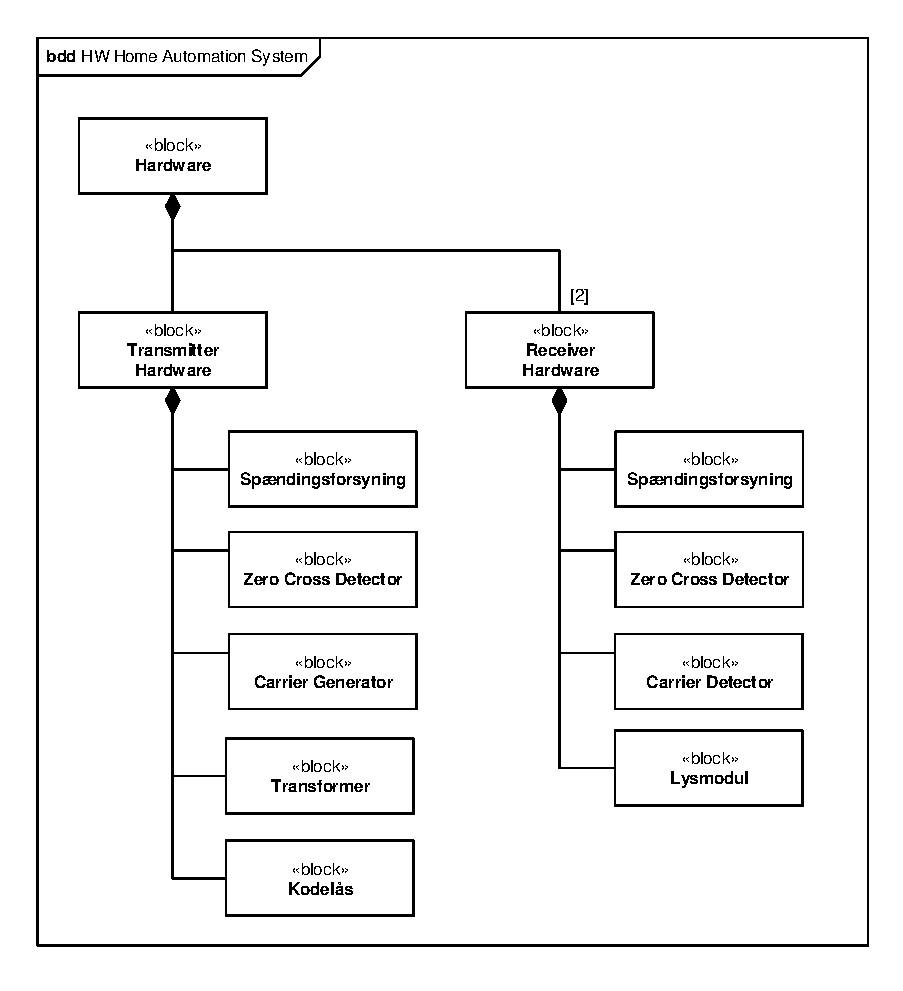
\includegraphics[scale=0.8, trim=10 10 10 10, clip=true]{../Projektdokumentation/HardwareDesign/Diagrammer/BDD_HW.pdf}
	\caption{BDD-diagram over hardware}
	\label{fig:HWBDD}
\end{figure}



Systemets hardware er opdelt i en transmitter- og to receiverdele. De underblokke, der optræder flere steder i systemet, er ens, og kan derfor betragtes som "byggeklodser", der hver har deres meget specifikke funktionalitet.Fordelen ved at opdele i byggeklodser, skal optræde flere steder i designet og derved undgås dobbeltarbejde. Hver underblok er kun beskrevet en gang. 

\subsection{Underblokke}

\subsubsection{Transformer}
Transformeren transformerer $230VAC$ til $18V AC$, og simulerer derved et almindeligt $230V$ el-net, der er sikkerhedsmæssigt forsvarligt at arbejde med.

\subsubsection{Spændingsforsyning}
Spændingsforsyningen anvendes i både transmitter- og de to receiver-blokke, hvor den genenerer ($12V$ og GND) til hhv. $+5V$ og $-5V$.\\

Oprindeligt blev spændingsforsyningen designet således, at den kun leverede $+5V$, men det blev erfaret under implementeringen, at bl.a. Zerocross Detektoren havde brug for $-5V$.\\

Der anvendes en fastspændingsregulator($LM7805$)\cite{lib:LM7805} og en spændings-inverter($ICL7660$)\cite{lib:IC7660}, der begge er opsat jf. standardapplikationen i deres respektive datablade. Kredsløbets færdige design kan ses på Figur \ref{fig:Stromforsyning}.

\begin{figure}[h]
	\centering
	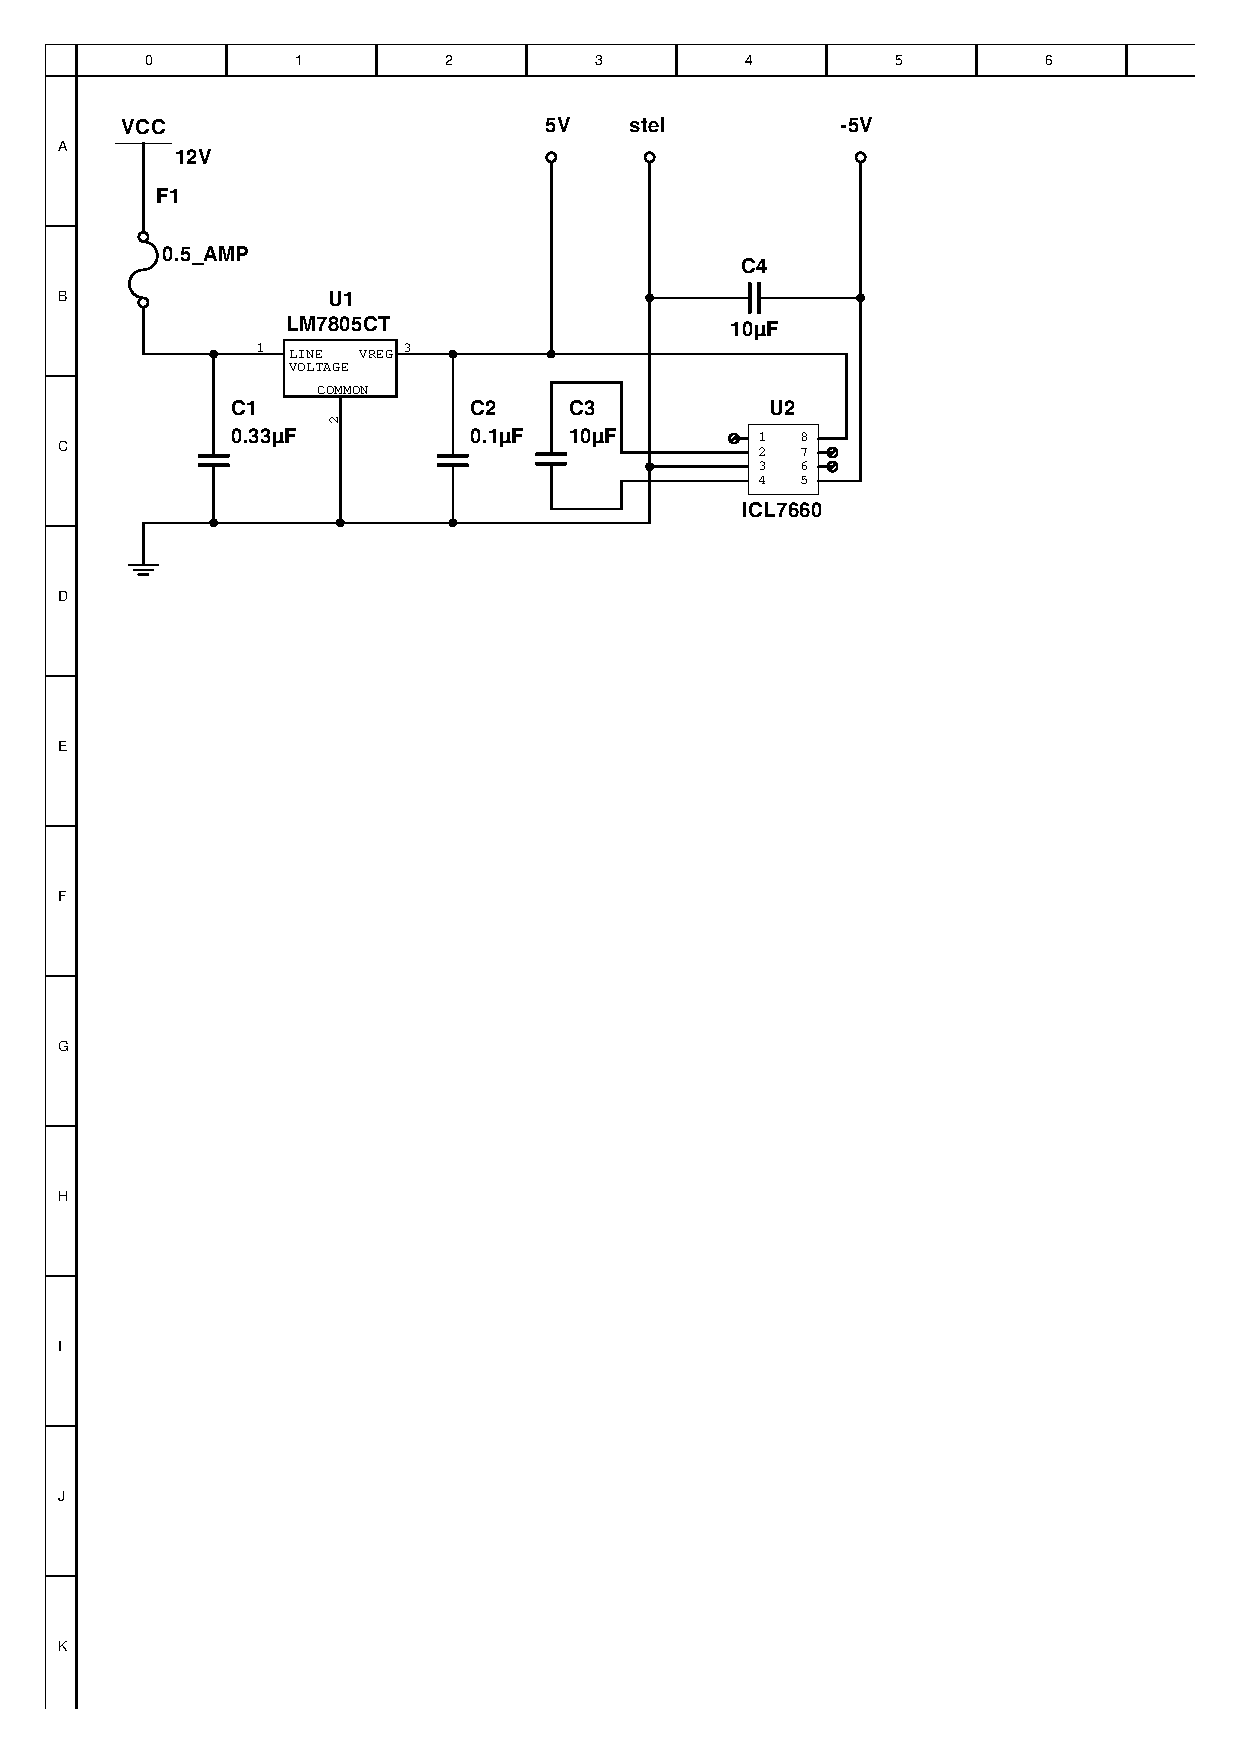
\includegraphics[scale=1,trim=50 555 150 50, clip=true]{../Projektdokumentation/HardwareDesign/Diagrammer/Stroemforsyning.pdf}
	\caption{Spændingsforsyning}
	\label{fig:Stromforsyning}
\end{figure}

En modultest af spændingsforsyningen viser at der leveres hhv. $+5.0V$ og $-5.0V$ på de respektive udgange.

\subsubsection{Kodelås}
Kodelåsen har til formål at forhindre adgang til systemet, såfremt der ikke er indtastet tre korrekte koder på DE-2 boardet, hvor kodelåsen er implementeret. Hvis der indtastes en forkert kode tre gange, vil kodelåsen låse for adgang til systemet permanent. Selve komponenten er lavet under en øvelse i faget Digital System Design og funktionaliteten er derfor ikke beskrevet yderligere.\\

Modultest og integrationstest viser at kodelåsen virker efter hensigten. Desuden er der i dokumentationen på side \pageref{P-sec:Kodelaas} gjort rede for, at udgangsspændingen ved logisk HIGH på DE2 boardet, er høj nok til at STK500-kittet registrerer det som logisk HIGH.

\subsubsection{Zerocross Detector}
Zerocross detector'en har til formål at detektere, hvornår der er en nulgennemgang på $50Hz$ nettet. Altså hvornår spændingen krydser nul. Denne information anvendes til at time hvornår der skal sendes $120kHz$ ud på $50Hz$ nettet, samt hvornår der skal læses. Når der detekteres en nulgennemgang på indgangen \textit{signal}, skal kredsløbets udgang \textit{ZeroCrossDetect} toggle mellem $0V$ og $5V$. Til at løse denne opgave er der designet et kredsløb, som vist på Figur \ref{fig:ZeroCrossDetect}.

\begin{figure}[h]
	\centering
	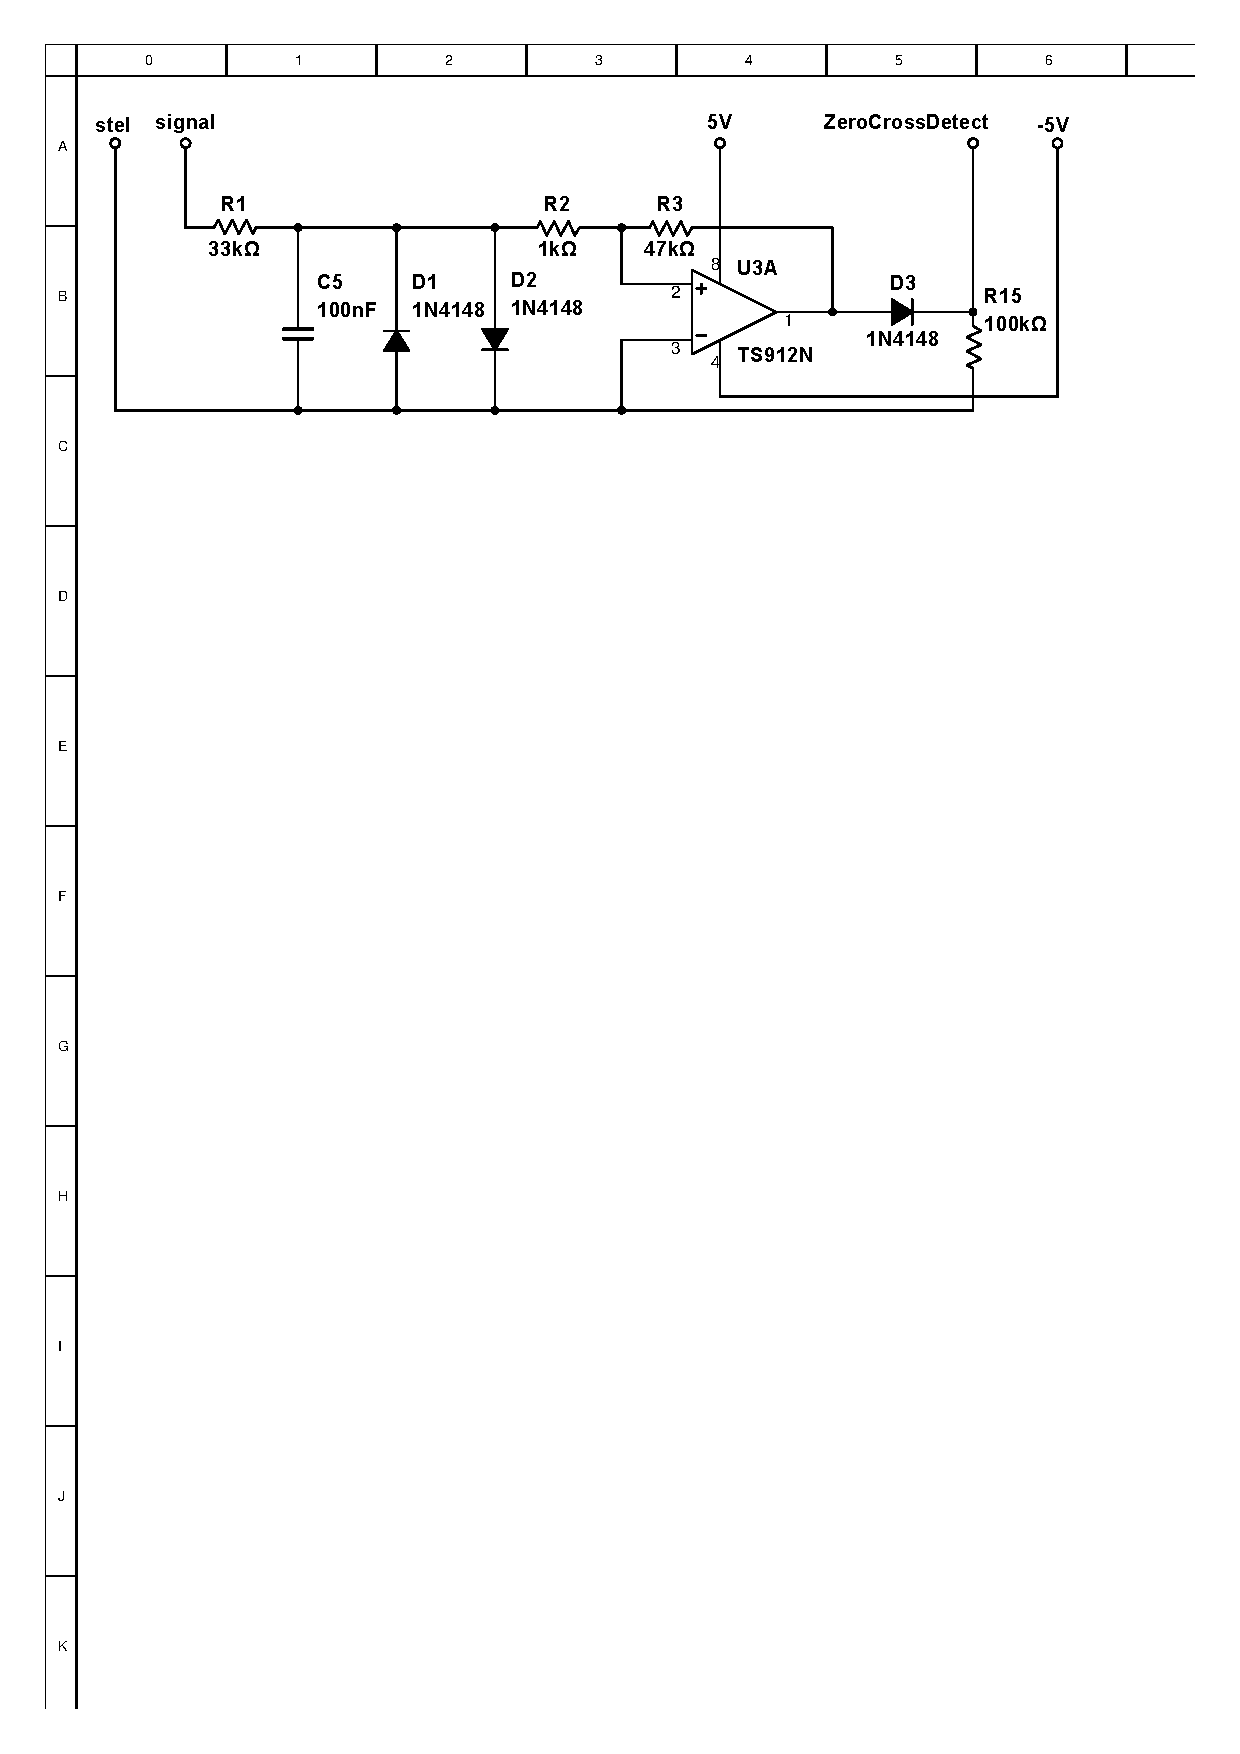
\includegraphics[scale=1, trim=45 635 80 50, clip=true]{../Projektdokumentation/HardwareDesign/Diagrammer/ZeroCrossDetector.pdf}
	\caption{Zerocross detector}
	\label{fig:ZeroCrossDetect}
\end{figure}

Kredsløbet består fra venstre mod højre af et lavpasfilter, to dioder\cite{lib:1N4148} til at begrænse spændingen, en operationsforstærker opsat som komparator med hysterese, en ensretter og en pull-down-modstand.\\

Det er valgt at bruge et lavpasfilter for at forhindre de $120kHz$, som også vil være til stede på \textit{signal}, i at genere kredsløbet ved at skabe ekstra nulgennemgange. Dioderne $D_{1}$ og $D_{2}$ begrænser spændingen til ca. $0.7V$, så vi ikke risikerer at ødelægge operationsforstærkeren ved at sende hhv. $\pm 25V$ ind på den.\\
Vi har valgt at bruge operationsforstærkeren TS912N, da denne kan forsynes med hhv. $\pm 5V$. Operationsforstærkeren\cite{lib:TS912} er opsat som komparator, således at den har $+5V$ på udgangen, hvis spændingen på plusbenet er højere end spændingen på minusbenet(referencespændingen), der er sat til $0V$. Hvis spændingen på plusbenet er lavere end referencespændingen, vil udgangen have en spænding på $-5V$. Der er tilføjet en hysterese med en passende størrelse ved hjælp af $R_{2}$ og $R_{3}$, for at undgå prel på operationsforstærkerens udgang.\\
Dioden $D_{3}$ ensretter strømmen, således at spændingen ikke kan blive negativ. Pull-down-modstanden $R_{15}$ trækker spændingen til $0V$, når udgangen på operationsforstærkeren er negativ, da det under implementering viste sig at være nødvendigt. Uden pull-down-modstand var signalet \textit{ZeroCrossDetect} ikke stabilt.\\

Efter de få nævnte tilpasninger, viste modul- og integrationstest, at kredsløbet virkede efter hensigten.

\newpage

\subsubsection{Carrier Generator}
Dette kredsløb har til formål at sende $120kHz$ signalet ud på $50Hz$ nettet. Dette skal ske uden at trække en væsentlig mængde strøm fra det STK500-kit, der generer de $120kHz$. Kredsløbets design vises på Figur \ref{fig:CarrierGen}. \\

\begin{figure}[h]
	\centering
	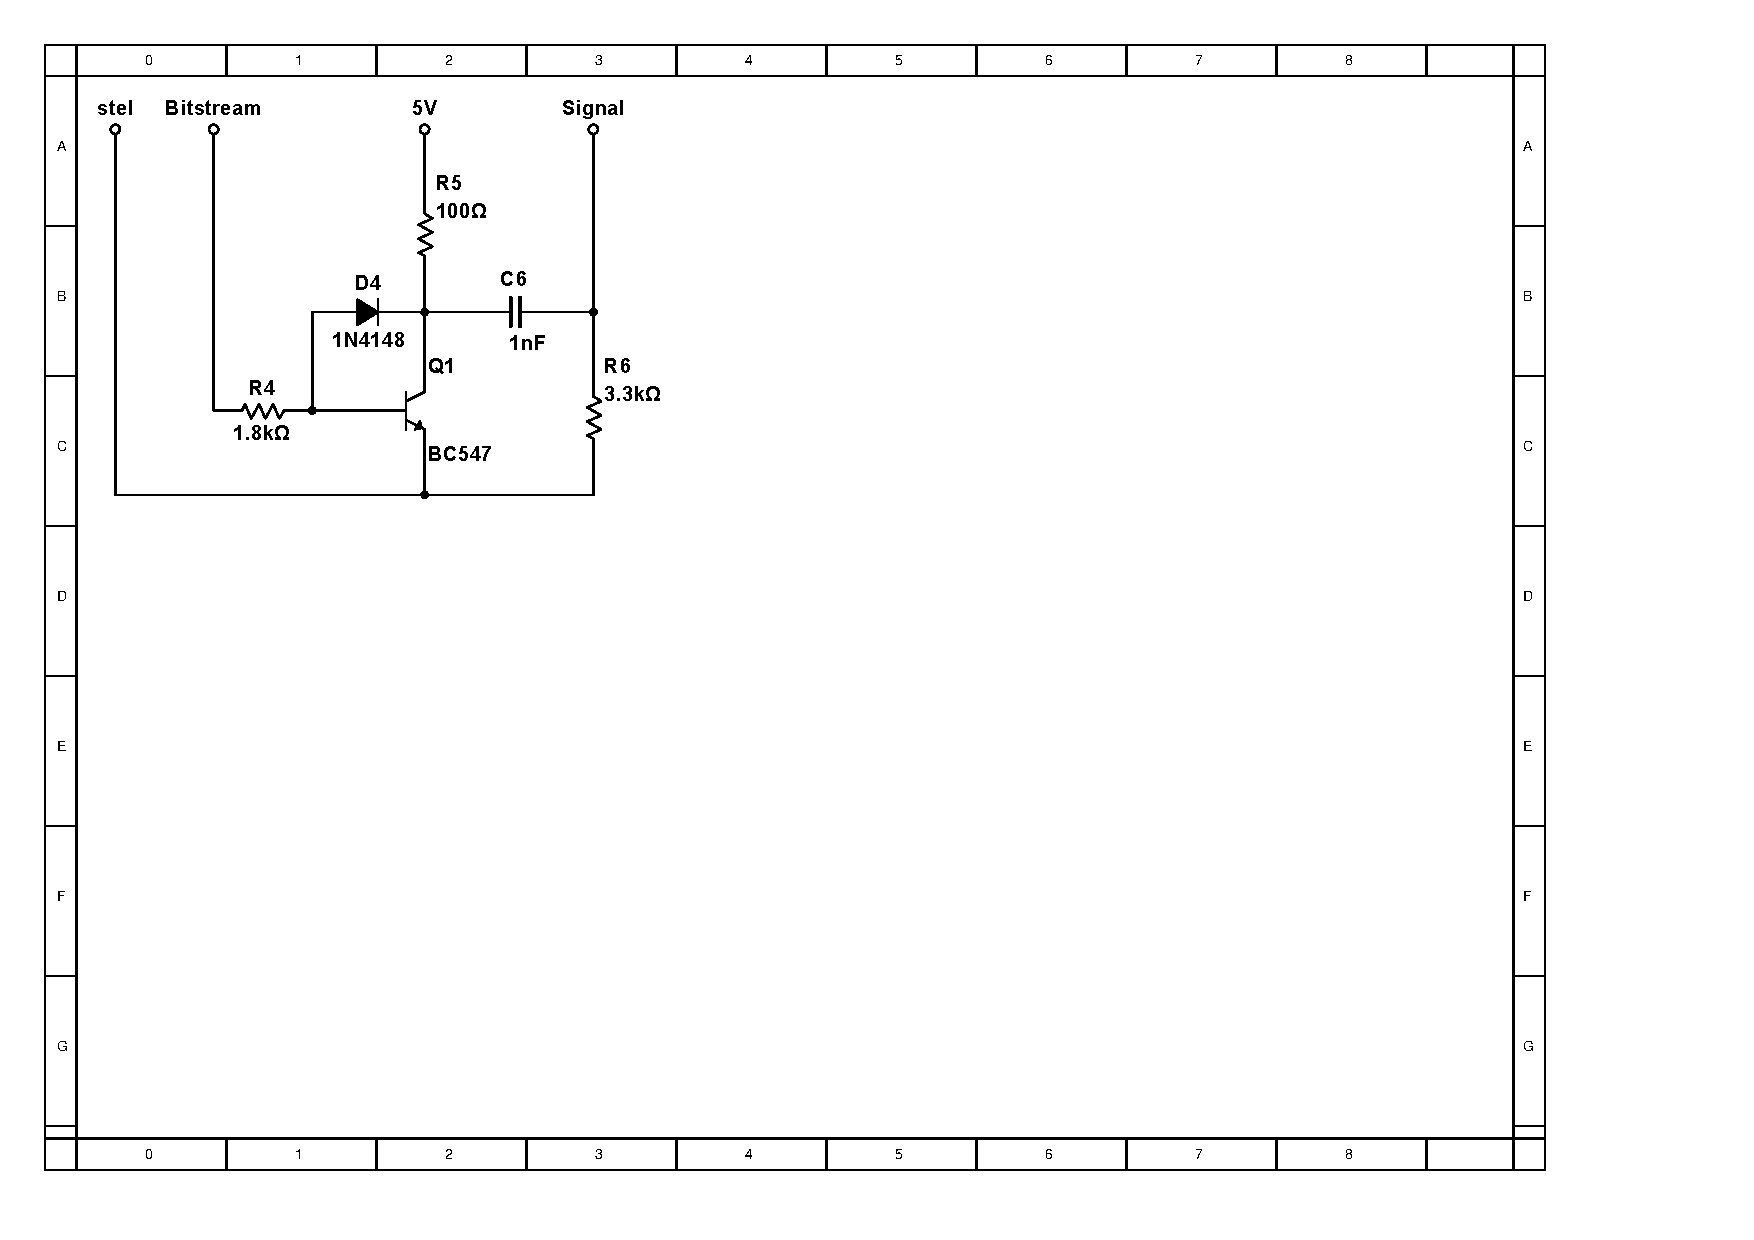
\includegraphics[scale=0.9, trim=45 355 525 45, clip=true]{../Projektdokumentation/HardwareDesign/Diagrammer/CarrierGenerator.pdf}
	\caption{Carrier generator}
	\label{fig:CarrierGen}
\end{figure}

Kredsløbet består af et transistor-kredsløb\cite{lib:BC547} og et højpasfilter($C_{6}$ og $R_{6}$). Højpasfilteret sikrer at transistor-kredsløbet ikke generes af $50Hz$ nettet, men $120kHz$ signalet, kan passere frit igennem. Transistor-delen, sørger for at åbne og lukke, for adgang til stel, i samme frekvens som \textit{Bitstream}, da transistoren er i mætning, hvilket bevirker at der er samme frekvens på collectorbenet som på basebenet af transistoren, men at strømmen trækkes fra $5V$ benet.\\

Transistoren BC547 er valgt, da denne har et lille storage delay. Målinger under implementeringen viste, at en positiv ladning af den transistor, der oprindeligt blev anvendt(BC139) ikke kunne nå at aflade, inden næste periode af $120kHz$ signalet skulle passere. Dioden $D_{4}$ hjælper ligeledes med at aflade den positive opladning af transistoren. Der er tale om en såkaldt baker clamp \cite{lib:BakerClamp}.\\

En modultest viser, at når \textit{Bitstream} har passeret gennem hele kredsløbet, er der påtrykt et $120kHz$ signal på $50Hz$ nettet. Signalet er ikke et ''pænt'' firkantsignal længere, og det har ikke en amplitude på $5V$, grundet diverse spændingsfald. Dette har ikke nogen betydning grundet carrier detectorens design. Der henvises i øvrigt til side \pageref{P-fig:CGImpl1} i projektdokumentationen for hele modultesten.\\

\newpage

\subsubsection{Lysmodul}
Lysmodulet har til formål at styre lysstyrken af en LED ved hjælp af pulsbreddemodulation (PWM). Dette gøres ved hjælp af en transistor\cite{lib:BD139} i mætning, således at middelstrømmen kan styres igennem LED'en, uden at strømmen trækkes fra STK500-kittet, som leverer \textit{lightPWM}-signalet. Kredsløbet er vist på Figur \ref{fig:Lysmodul-kredslob}.\\

\begin{figure}[h]
	\centering
	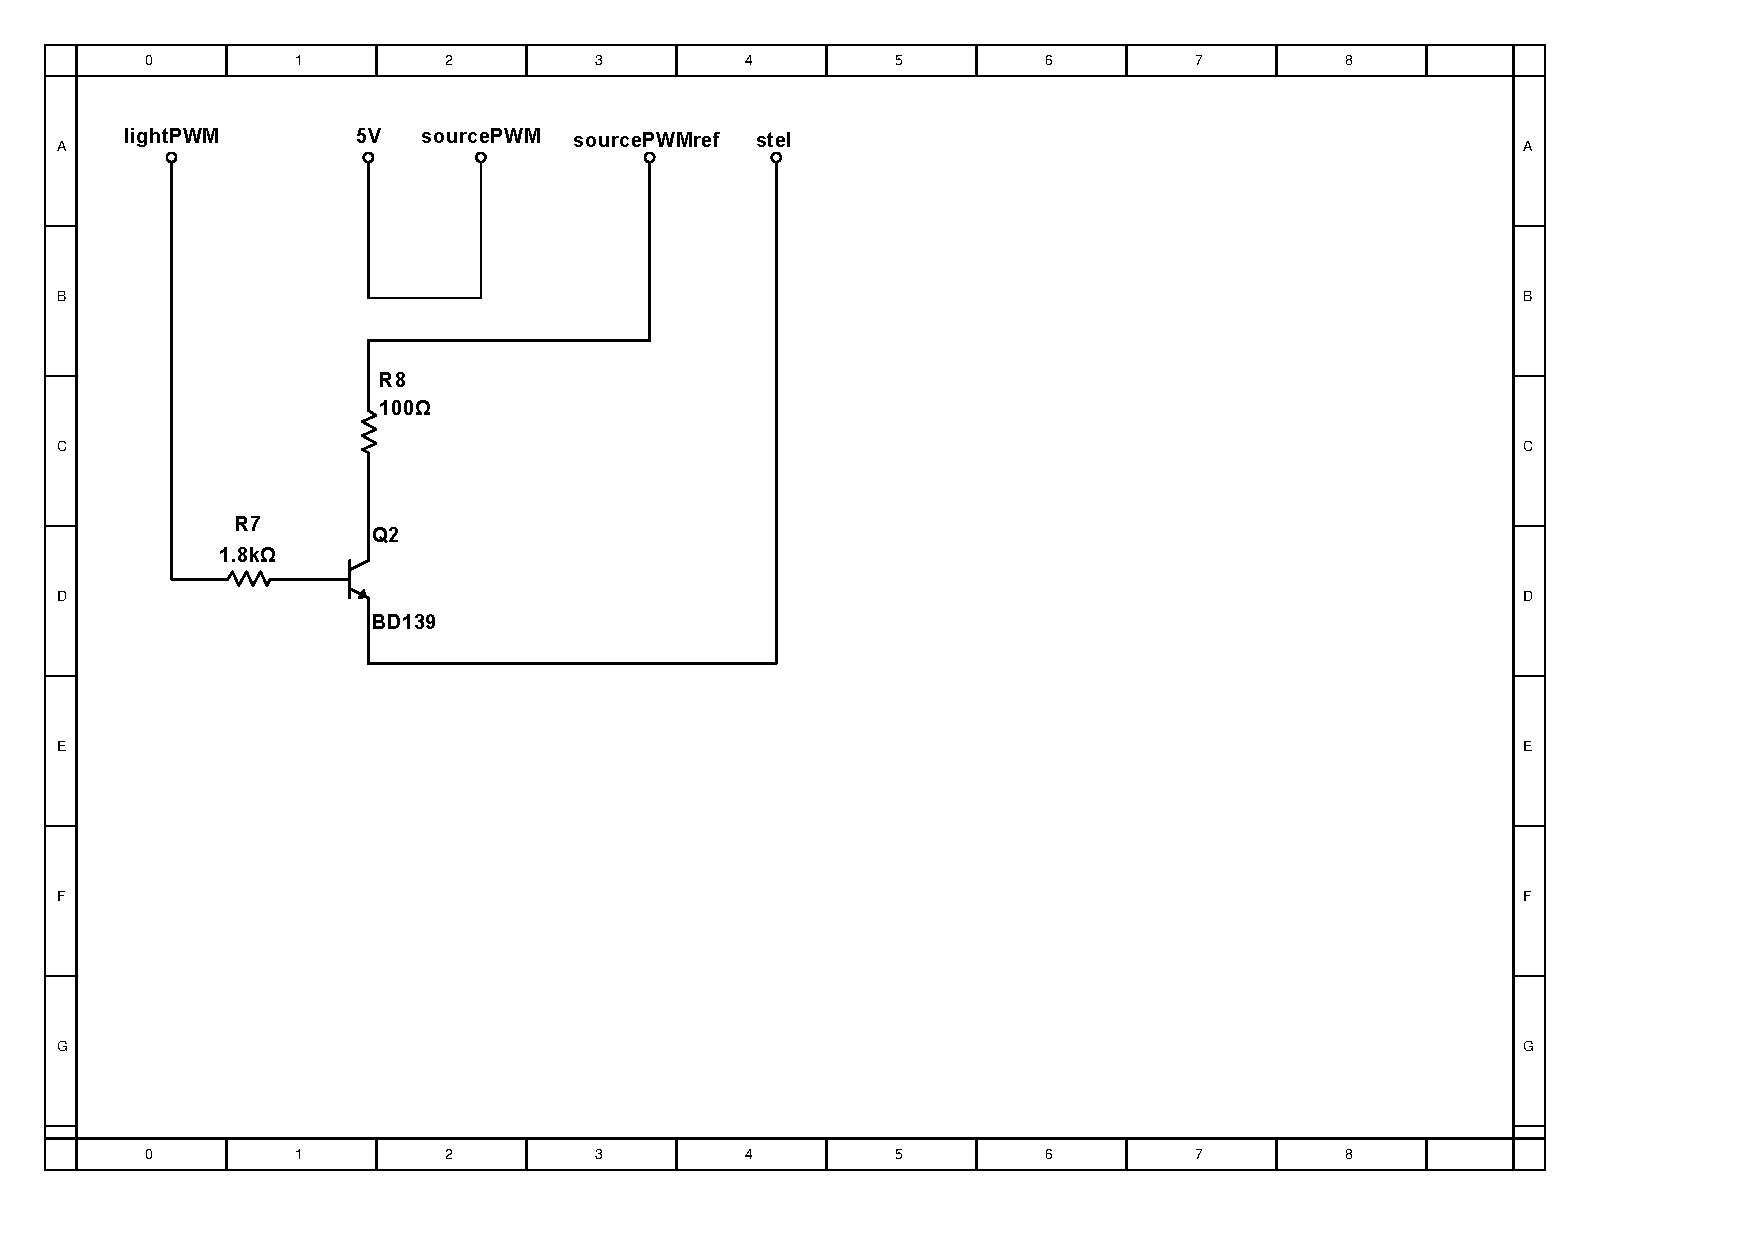
\includegraphics[scale=0.8, trim=50 250 440 60, clip=true]{../Projektdokumentation/HardwareDesign/Diagrammer/Lysmodul.pdf}
	\caption{Lysmodul}
	\label{fig:Lysmodul-kredslob}
\end{figure}

På terminalerne \textit{sourcePWM} og \textit{sourcePWMref}, tilsluttes den eksterne LED\cite{lib:LED}, som beskrevet i systemarkitekturen i projektdokumentationen på side \pageref{P-subsec:IBDX10Lys}.\\

Modul- og integrationstest af komponenten viser, at der tydeligt kan ændres i lysstyrken ved at ændre på duty cycle'en.\\

\newpage

\subsubsection{Carrier Detector}
Carrier detector'en har til formål at detektere, om et $120kHz$ signal er til stede på $50Hz$ nettet. Når et $120kHz$ signal er til stede på \textit{signal}, er udgangen \textit{Bitstream} HIGH, og hvis der ikke er et $120kHz$ signal til stede, er udgangen LOW. Kredsløbet er vist på Figur \ref{fig:CarDetek}.

\begin{figure}[h]
	\centering
	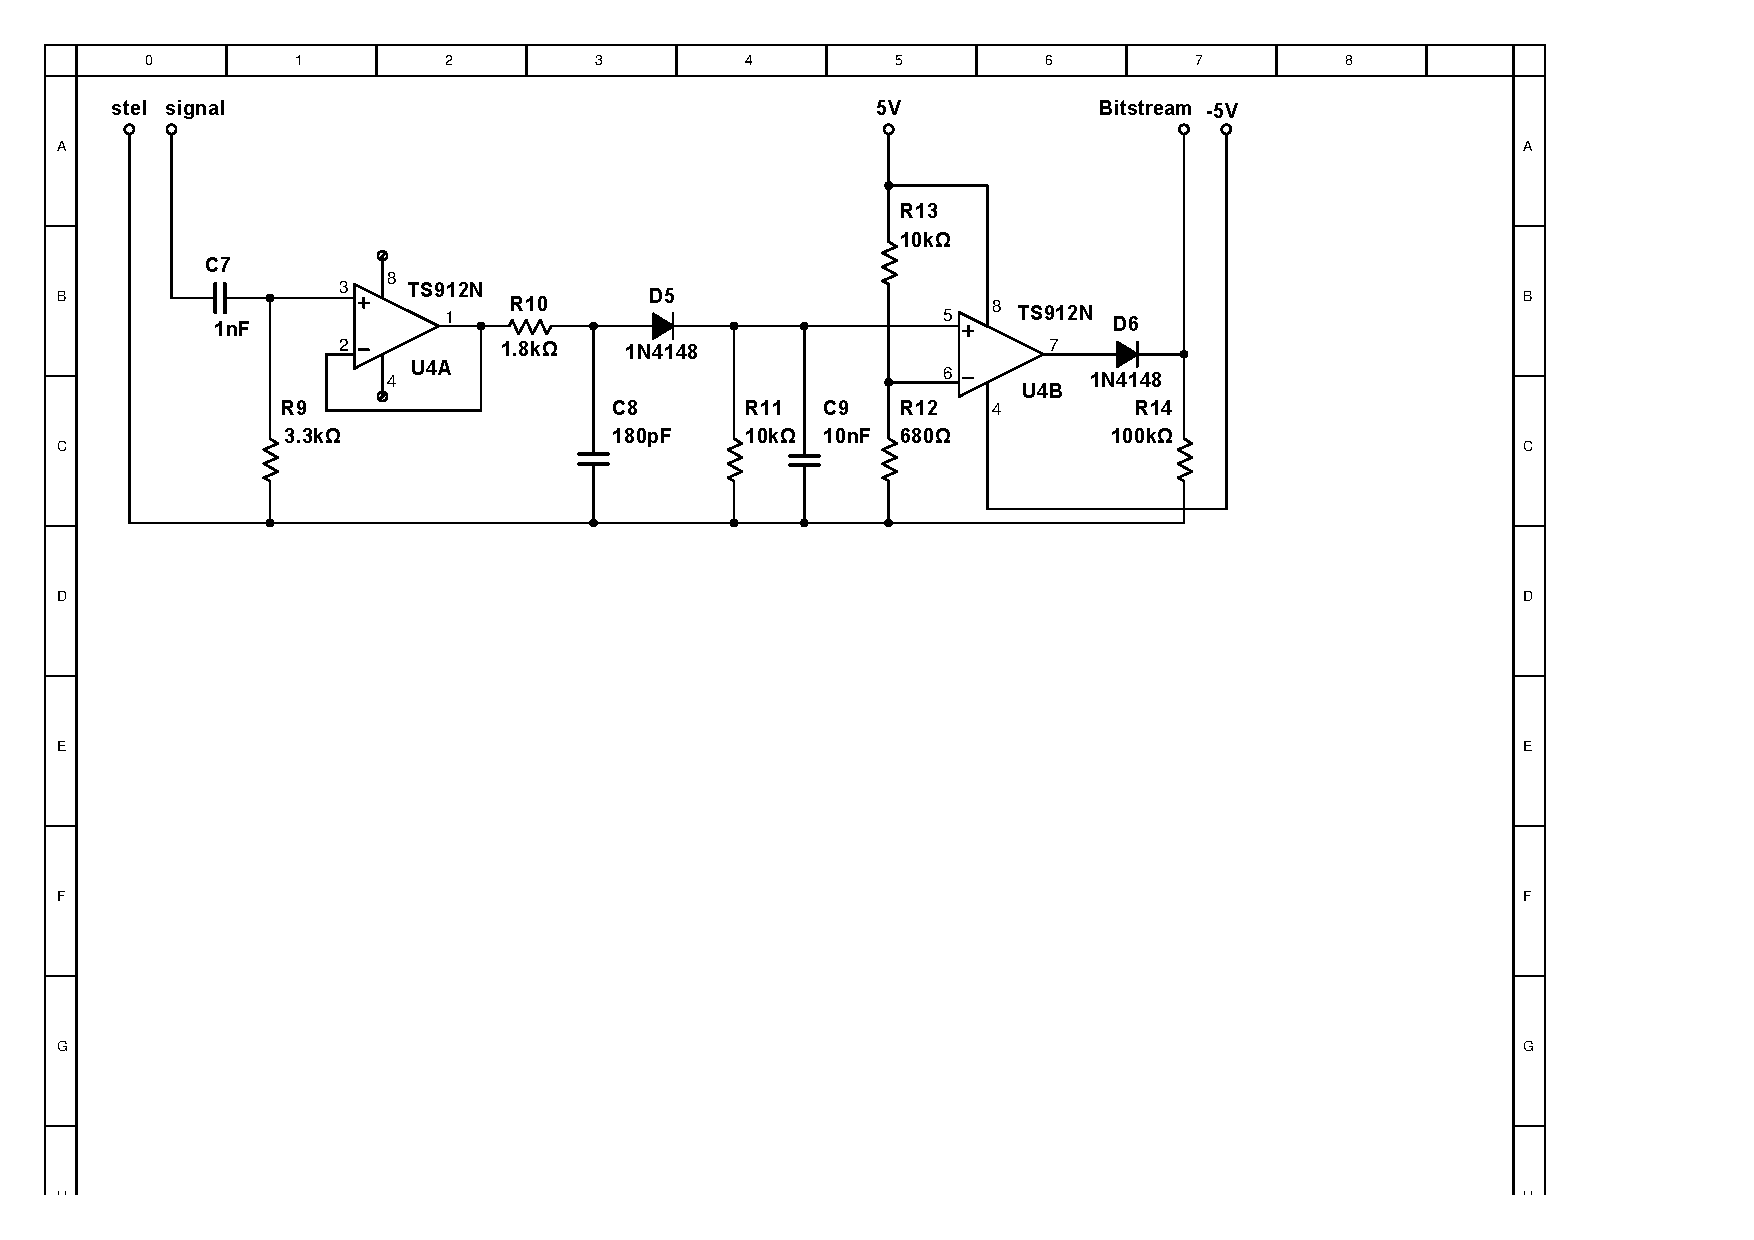
\includegraphics[width=\textwidth, trim=40 340 240 40, clip=true]{../Projektdokumentation/HardwareDesign/Diagrammer/CarrierDetector.pdf}
	\caption{Carrier detector}
	\label{fig:CarDetek}
\end{figure}

Fra venstre mod højre består kredsløbet af et båndpasfilter, en envelope detector, en operationsforstærker\cite{lib:TS912} opsat som komparator, en diode som ensretter og en pull-down-modstand.

Båndpasfilteret er designet, så det dæmper alle frekvenser på nær dem der ligger mellem $50kHz$ og $500kHz$, således at det frasorterer $50Hz$ og lader $120kHz$ passere. Da der er tale om et båndpasfilter, vil det også frasortere evt. højfrekvent støj, og evt. andre frekvenser end grundfrekvensen i $120kHz$ signalet. Det vil således være en tilnærmelsesvis sinus/cosinus, på $120kHz$, der lukkes igennem filteret.

Envelope detector'en består af $D_{5}$\cite{lib:1N4148}, $R_{11}$ og $C_{9}$ og har til opgave at holde spændingen omkring den positive peak-værdi, der er på $120kHz$ signalet. Dioden ensretter strømmen, således at det kun er positive spændinger der kan passere. Hvert peak af inputtet vil oplade kondensatoren, der sørger for, at spændingen i punktet mellem dioden og kondensatoren holdes nær peakværdien. Modstanden i parallel med kondensatoren vil gradvist aflade kondensatoren. Størrelserne på kondensatoren og modstanden er afpasset således, at afladningen sker i et passende tempo.

Operationsforstærkeren\cite{lib:TS912} er designet som en komparator, der har en udgangsspænding på $+5V$, når spændingen på ikke inverterende indgang er højere end spændingen på den inverterende indgang(referencespændingen). Når spændingen på ikke inverterende indgang derimod er mindre referencespændingen, er udgangsspændingen $-5V$. Referencespændingen er fastsat til en passende værdi, så spændingen på den ikke inverterende indgang kun er over spændingen på den inverterende indgang, når envelope detectoren detekterer et $120kHz$ signal.

Efter komparatoren er der placeret en diode $D_{6}$\cite{lib:1N4148}, som fungerer som ensretter, og en pull-down-modstand $R_{14}$, så der fremkommer et signal, der er i overensstemmelse med systemarkitekturen.

Modul- og instrumentationstest har vist, at komponenten virker efter hensigten. Spændingen på udgangen \textit{Bitstream} er ca. $4.7V$, når der er $120kHz$ til stede på \textit{signal}, og $0.0V$ når der ikke er $120kHz$ til stede på \textit{signal}.